\chapter{Introduction}
\thispagestyle{empty}
\section{Autonomous Surface Vehicles: challenges and applications}
Unmanned Surface Vehicles (\textbf{USVs}) are particular surface vessels capable of navigating without the presence of a human crew to maneuver them. They can be \textit{remotely operated} through radio or satellite communication, or be completely \textit{autonomous} and controlled by a computer or artificial intelligence; in this case, they are referred to as \textbf{Autonomous Surface Vehicles (ASVs)}. ASVs aim to make journeys \textit{safer}, \textit{reduce costs}, \textit{increase operational continuity}, and carry out \textit{prolonged missions} in \textit{complex} and even \textit{risky} situations for humans.\\

All this has been made possible thanks to significant technological evolution in \textbf{sensors} (satellite, IMU, cameras, LIDAR, radar, etc.), major developments in \textbf{robotics libraries}, and onboard \textbf{computational power} that is increasingly greater and more affordable. Despite this, the \textbf{marine environment} presents major challenges. For example, the \textit{plane of the sea surface} is not a fixed reference but changes independently of the boat’s movements; the surface creates \textit{reflections} that can interfere with instrumentation; and \textit{wind and waves} can put stability control systems to the test. In the marine context, therefore, \textbf{attitude estimation} (roll, pitch, and yaw) is essential, as it is decisive both for the \textit{success of the journey} and for the \textit{precision required in maneuvers}, such as docking.\\

The main challenges concern \textbf{sensors and algorithms}. The first challenge involves \textbf{navigation with GNSS} (Global Navigation Satellite System), which degrades in proximity to port infrastructures, bridges, or areas with many vertical obstacles, as part of the visible satellites are lost. This problem has been partly mitigated with \textbf{inertial sensors (IMU)}, which, however, suffer from another issue: \textit{drift}. The second challenge is the \textbf{detection of possible obstacles} at sea, such as buoys, debris, or even other vessels, often under conditions of \textit{reduced visibility} or \textit{reflections}. The third challenge is \textbf{control and stability}, made complex by \textit{wave motion} that often causes very rapid variations. The last challenge is the ability to make \textbf{real-time decisions}, including very quick changes dictated by sudden shifts in the operational situation.\\

Despite the criticality of these challenges, ASVs are used in various \textbf{applications}. In the \textbf{industrial field}, they are employed for \textit{infrastructure inspection} or \textit{short-range logistical support}. In \textbf{defense and security}, they are used in \textit{special operations} such as \textit{explosive ordnance disposal}. In the \textbf{environmental field}, they are used for \textit{monitoring environmental parameters} and \textit{collecting meteorological data} over extended time horizons, thereby reducing risks for crews.\\

Within this framework, the present thesis focuses on one main issue: obtaining an \textbf{accurate real-time estimation} of the boat’s attitude. To achieve this, \textbf{computer vision techniques} (stereo vision and ArUco markers), \textbf{inertial measurements} through the IMU, and an \textbf{Extended Kalman Filter} will be used to fuse the data, with the aim of \textit{improving the reliability of the estimation}.

\section{Attitude Estimation: roll, pitch, yaw}

To describe the \textbf{attitude} of a vessel, the orientation of the rigid body with respect to a reference system is used. This is done through the three \textbf{Euler angles}\cite{Euler_angles}: \textit{roll} (rotation on the longitudinal axis), \textit{pitch} (rotation on the transverse axis), and \textit{yaw} (rotation on the vertical axis). These three quantities are \textbf{crucial} as they influence \textbf{stabilization} and \textbf{trajectory control} and are fundamental in \textbf{precision maneuvers}.  

\begin{figure}[ht]
  \centering
  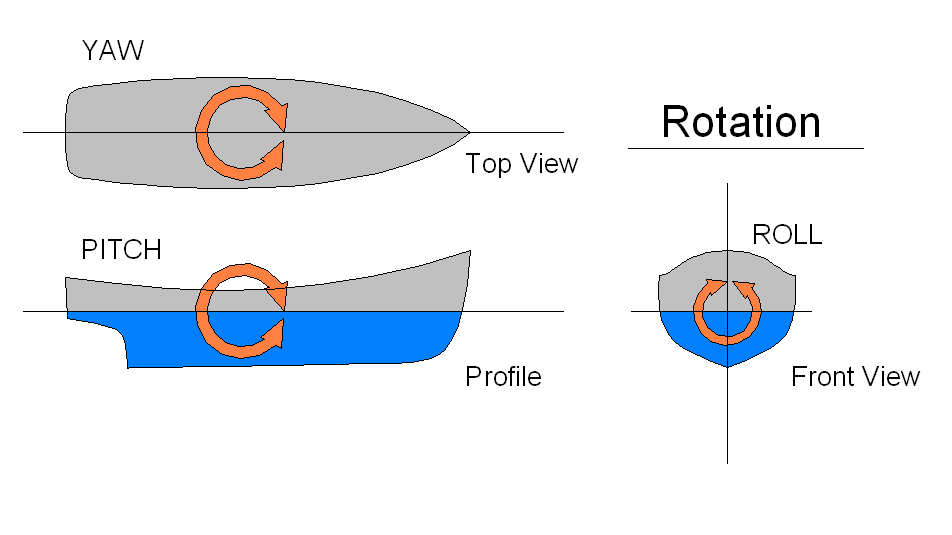
\includegraphics[height=6cm]{images/euler_angles.png}
  \caption{Three rotational degrees of freedom of a ASV}\label{unipd-logo}
\end{figure}


\textbf{Attitude estimation} can be obtained from different sources, each with its own advantages and disadvantages. \textbf{Inertial sensors (IMU)}\cite{IMU_Euler}, through gyroscopes and accelerometers, provide roll and pitch with a \textbf{high update frequency}. However, these estimates are affected by \textit{drift}, caused by the accumulation of errors over time. For yaw, a \textbf{magnetometer} or an \textbf{external observation} is required, as the IMU does not provide a direct measurement of this angle. A \textbf{visual sensor} allows estimating the attitude through \textit{known structures} (e.g., ArUco tags) or through the environment if it allows it (e.g., using the \textit{horizon line}). This latter method is less affected by the drift problem but is highly sensitive to \textbf{environmental conditions} and also has a \textbf{lower update frequency}.  

In the \textbf{marine context}, a robust pipeline is represented by the IMU, which provides a \textbf{high-frequency prediction} and, periodically, through \textbf{computer vision}, a measurement relative to the ArUco marker to reduce error accumulation. Through an \textbf{EKF filter}\cite{EKS_IMU_cv}, the different contributions are integrated in order to obtain a \textbf{coherent estimate} even if the conditions are adverse or if one of the sources fails.  

In summary, \textbf{attitude estimation} for an \textbf{ASV} requires a compromise between the \textbf{speed of the readings} and their \textbf{accuracy}. The \textbf{integration} between \textit{inertial} and \textit{visual} measurements provides a \textbf{reliable estimate} capable of supporting \textbf{autonomous navigation}. Subsequently, the different \textbf{implementation choices} to obtain the attitude estimation of the \textbf{Blue Boat} will be presented.  

\section{Computer Vision for Localization and Attitude Estimation}

Computer vision is an essential source for estimating the attitude of the ASV. 
It provides \textbf{roll}, \textbf{pitch}, and \textbf{yaw} with respect to a known reference, 
namely the \textit{ArUco marker}. In our case, it plays a \textit{complementary role} with respect to the IMU, 
which provides an absolute measurement that is not obtained through temporal integration, 
but is instead sensitive to visual conditions (\textit{reflections, backlighting, fog, etc.}).\\
The goal of this chapter is to outline the principles and choices that allow for reliable 
attitude estimation using a \textbf{stereo camera pair}, leveraging \textit{ArUco markers} 
and a geometric calibration of the two cameras.\\

The pipeline is structured into four main steps:
\begin{itemize}
    \item \textbf{Stereo camera calibration:} estimation of intrinsic parameters and distortions, 
    followed by the calculation of rotation and translation between the two cameras.
    \item \textbf{Marker detection:} ArUco markers enable highly reliable identification, 
    provided they are properly scaled according to the distance and have a sufficient pixel resolution.
    \item \textbf{Attitude estimation:} application of a pose estimation algorithm which, 
    knowing the 2D corners and the 3D points of the pattern, can estimate the values of roll, pitch, and yaw.
    \item \textbf{Measurement validation:} a decision filter determines whether to accept the measurement, 
    discard it, or reduce its influence.
\end{itemize}

Triangulation, made more reliable by \textbf{epipolar rectification}, allows for the estimation of depth around the marker. 
These depth cues are used as additional support to improve the attitude estimation.\\

Finally, temporal and synchronization aspects also play a \textbf{crucial role}. 
Synchronization is \textit{decisive} to avoid disparities and inconsistent triangulations. 
The frame rate and the subsequent update time strongly influence the \textbf{accuracy} of the algorithm’s estimation, 
since excessively low values reduce its quality.\\

This approach, entirely based on stereo vision and ArUco markers, enables precise attitude estimation. 
Its accuracy is determined by the quality of calibrations and the robustness of estimation algorithms, 
but it reaches its maximum effectiveness when \textbf{integrated with IMU data}, 
compensating for the weaknesses of each source.

\section{Fiducial markers and ArUco tags}

The \textbf{ArUco marker} is a square planar pattern with a high-contrast black border and an internal matrix encoding a \textit{unique identifier}. This structure allows for fast localization and recognition of the four corners, providing a stable 2D--3D correspondence for attitude estimation. The use of a single marker reduces environmental and economic requirements. However, relying on just one marker requires greater care in localization, calibration, and validation of the measurements.\\

The recognition pipeline adopts a pair of calibrated cameras. After calibration of the individual cameras and subsequent stereo calibration (\textit{rotation, translation, and epipolar rectification}), the images are acquired and rectified, thus aligning the epipolar lines. The detection of the marker involves several steps:

\begin{enumerate}
    \item Adaptive thresholding
    \item Contour extraction
    \item Quadrilateral selection
    \item ID decoding\\
\end{enumerate}

Knowing the marker size, the attitude is calculated through the \textbf{PnP algorithm (Perspective-n-Point)}, obtaining the rotation and translation of the reference camera frame. If both cameras observe the marker, the two estimates can be fused, or the one with higher quality can be selected.\\

The use of a system based on \textbf{stereo vision} improves disparity estimation in the regions close to the marker and enables \textit{metric triangulation} of depth, enhancing stability compared to a monocular approach. This becomes particularly evident when the marker is very small (i.e., far away) or when it is not perpendicular to the viewing angle, as both conditions reduce perspective information.\\

For each estimate, quality indicators are evaluated: reprojection error, effective presence of the marker (all four corners detected), and the angle between the camera and the marker, penalizing views that are too oblique. Furthermore, a comparison is made between the apparent size of the marker in pixels, in order to identify discrepancies due to triangulation or temporal misalignment. \\

From a practical point of view, the use of a single ArUco marker offers a \textbf{simple and easily reproducible implementation path}: a single print on a rigid surface with a matte finish (to reduce reflections) is sufficient. Under these conditions, a single ArUco marker used in a well-calibrated stereo vision pipeline provides roll, pitch, and yaw measurements while maintaining a \textit{good trade-off between precision and computational demand}.
\section{Sensor Fusion and Bayesian Approaches}

Sensor fusion deals with solving the problem of combining \textbf{heterogeneous and noisy measurements} in order to obtain a state estimate that is more accurate than the one provided by individual sensors.  
In our case, we merge sensors with \textbf{complementary properties}:  
\begin{itemize}
    \item \textbf{Stereo vision} provides \textit{absolute measurements} without drift but at a low frequency.  
    \item \textbf{IMU} provides \textit{angular velocity} measurements at high frequency but suffers from drift.  
\end{itemize}

\subsection*{Bayesian Foundations}
In the \textbf{Bayesian paradigm}, the state is described by a \textit{probability distribution} that evolves over time and is composed of two steps:  
\begin{itemize}
    \item \textbf{Prediction:} computes the next step based on the dynamic model and the noise statistics.  
    \item \textbf{Update:} uses the available measurement through the observation function and the measurement noise statistics.  
\end{itemize}

This alternation achieves an \textbf{optimal trade-off} between what is computed and what is \textit{effectively measured}.  

\subsection*{In our case, the requirements are:}
\begin{itemize}
    \item \textbf{State:} Euler angles (\textit{roll, pitch, yaw}).  
    \item \textbf{Dynamics:} integration of angular velocities to predict the evolution of the angles using consecutive samples.  
    \item \textbf{Observations:} an orientation measurement derived from vision and inertial measurements, which will be treated either as model input or as an observation depending on the architecture.  
\end{itemize}

It is necessary to guarantee a \textbf{numerical consistency} between prediction and update, managing, for example, the correct periodicity of measurements and possible discontinuities among angles.  

\subsection*{Benefits of Fusion}
\begin{itemize}
    \item \textbf{Drift reduction:} vision-based observation removes the accumulation of error caused by inertial integration.  
    \item \textbf{Temporal continuity of the IMU:} keeps the estimate stable since it has a high update frequency.  
    \item \textbf{Robustness:} weighting measurements based on their \textit{uncertainty} allows discarding unreliable measurements from stereo vision (e.g., camera at a steep angle relative to the ArUco marker, marker too small, etc.) or from the IMU.  
\end{itemize}

\subsection*{Evaluation}
The quality of the fusion evaluation is assessed based on:  
\begin{itemize}
    \item \textbf{Angular accuracy}  
    \item \textbf{Temporal stability}  
    \item \textbf{Behavior under varying visual quality}  
\end{itemize}

\subsection*{Summary}
In summary, \textbf{sensor fusion with a Bayesian algorithm} allows combining stereo vision and IMU measurements to obtain the attitude estimate.  
\begin{itemize}
    \item \textbf{IMU:} provides a \textit{continuous and fast estimate},  
    \item \textbf{Stereo vision:} provides an estimate that does not suffer from drift since it is anchored to fixed references.  
\end{itemize}

Weighting the measurements according to their uncertainty allows operation even when the \textbf{quality of observations is not uniform}.  

\section{Kalman Filters as Bayesian Filters (Linear and Extended)}

Kalman filters are part of the family of \textbf{Bayesian filters}; they recursively estimate the state of the system in a \textit{probabilistic} way and update it through a \textbf{dynamic model (prediction)} with new \textbf{observations (update)} using \textbf{Bayes’ theorem}. In linear cases with \textit{Gaussian noise of zero mean}, the \textbf{Kalman Filter (KF)} provides an \textbf{optimal solution} since it maintains the state described by mean and covariance, producing a \textbf{Kalman gain} that balances the model and the measurements. In \textit{nonlinear systems}, typical in robotics and computer vision, the \textbf{Extended Kalman Filter (EKF)} is used, which applies a \textbf{local linearization (Jacobian matrices)} of the models to preserve the prediction structure.  

In our case, to estimate the attitude, the minimum state includes the \textbf{Euler angles (roll, pitch, yaw)} and the \textbf{angular velocities}. The \textbf{prediction} integrates angular velocities over the sampling step. The \textbf{update} incorporates an \textit{orientation observation} coming from computer vision, with a covariance built from the \textit{quality indicators} of the stereo vision pipeline (reprojection error, number and quality of corners, etc.). In this case, the filter avoids \textbf{drift} caused by the inertial system if the computer vision part is stable.  

At the \textbf{operational level}, the \textbf{linear KF}, through known \textbf{transition and observation matrices}, calculates prediction and update. If the state is nonlinear, the \textbf{EKF} is used, which, through the calculation of \textbf{Jacobian matrices}, replaces constant matrices within the same recursive scheme. The success of the fusion depends on the \textbf{consistency of the measurements}, which in turn depends on \textbf{temporal synchronization} between computer vision and IMU measurement, as well as \textbf{good performance conditions} that allow everything to run \textit{in real time}, etc.  

In summary, the \textbf{Kalman Filter} and its \textbf{extended version}, through a \textbf{Bayesian approach}, perform \textbf{sensor fusion} in a \textbf{computationally efficient} way: the \textbf{prediction} exploits the \textbf{dynamic model} and the \textbf{IMU angular velocities} to ensure \textbf{continuity and responsiveness} in any situation, while the \textbf{update} also integrates \textbf{computer vision}, thus providing an \textbf{accurate and temporally stable attitude estimate}.  